

本章中构建的软件并不复杂——我们将创建一个简单的计算器,将两个数字相加(图12.1)。它将作为一个控制台应用程序发布,带有一个文本用户界面和一个用于执行数学运算的库,这可能用于其他项目。虽然在现实生活中这样的项目没有太多用处,因为C++在其标准库中为计算提供了大量支持,但它将完美地用于探索本书中讨论的所有技术如何在实践中协同工作:

\begin{center}
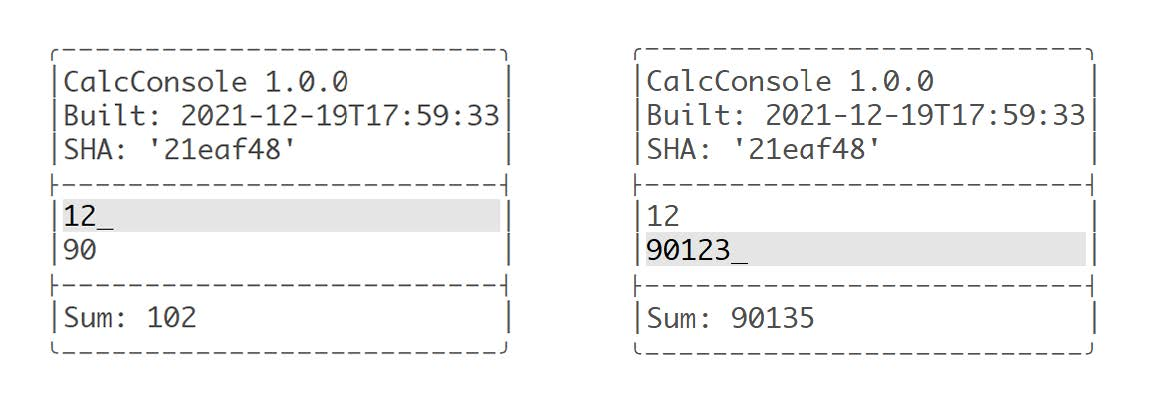
\includegraphics[width=0.8\textwidth]{content/3/chapter12/images/1.jpg}\\
图12.1 控制台计算器用户界面的两种状态
\end{center}

通常,项目要么生成面向用户的可执行文件,要么为开发人员生成库。同时具备这两种功能的项目比较少见——一些应用程序提供独立的SDK或库来支持插件,另一种情况可能是提供其用法示例的库。我们在本章中构建的项目在某种程度上属于最后一类。

这里先回顾一下之前章节的内容,并选择其中描述的技术和工具来构建我们的应用程序:

第1章:

提供关于CMake的基本信息——如何安装它,并使用命令行来构建项目。这里提供的有关项目文件的信息是关键:不同文件的职责、常规使用的名称,以及一些怪癖。本章中,还讨论了生成器的预设文件,但在本项目中先跳过这些文件。

第2章:

介绍了编写正确的列表文件和脚本所需的工具,分享了关于代码的基本信息:注释、命令调用和参数。我们还详细解释了变量、列表和控制结构,并给出了一些非常有用的命令。这些知识将应用于整个项目。

第3章:

这里的内容将对项目产生关键性影响:

\begin{itemize}
\item 
指定最低的CMake版本将决定,应用哪些CMake策略;命名、版本控制和配置项目语言会影响构建的基本行为。

\item 
了解形成目录和文件布局的项目分区和结构。

\item 
系统发现来帮助我们决定了如何处理不同的环境,特别是对于这个项目——例如,是否需要运行ldconfig?

\item 
工具链配置允许特定版本的C++和编译器支持的标准需求。
\end{itemize}

本章还说明了禁用源代码内构建通常是一个好主意。

第4章:

这里,强调了每个现代CMake项目是如何使用目标的,原因如下:

\begin{itemize}
\item 
定义一些库和可执行程序(用于测试和生产)将使项目保持有组织和DRY。

\item 
目标属性和传递性使用需求(传播属性)保持配置接近目标定义。

\item 
生成器表达式将在整个解决方案中出现,使它们尽可能简单。
\end{itemize}

这个项目中,将使用自定义命令为Valgrind和覆盖率报告生成文件,并且使用目标钩子(PRE\_BUILD),来清理覆盖率工具生成的.gcda文件。

第5章:

没有编译就没有C++项目,CMake允许我们以多种方式调整这个过程:扩展目标的源、配置优化器和提供调试信息。对于这个项目,默认的编译标志就可以了,但我们将继续使用预处理器:

\begin{itemize}
\item 
将在编译后的可执行文件中存储构建元数据(项目版本、构建时间和Git提交SHA),并将其显示给用户。
	
\item 
将启用头文件的预编译。在如此小的项目中,这并不是必须的,但它将帮助我们实践这个知识点。
\end{itemize}

统一构建将不是必要的——这个项目将不够大,但也可以添加。

第6章:

提供了关于链接的信息(在任何项目中都很有用),其中大部分在默认情况下很有用。但是由于这个项目也提供了一个库,将显式地引用以下的一些构建说明:

\begin{itemize}
\item 
用于测试和开发的静态库

\item 
要发布的动态库
\end{itemize}

本章概述了如何分离main()进行测试,我们的项目中也有测试。

第7章:

为了使项目更有趣,将引入一个外部依赖项:一个文本UI库。本章中描述了一些依赖管理方法。选择正确的一个并不太难:FetchContent实用程序模块通常是推荐的,也是最方便的(除非解决本章中描述的特定情况)。

第8章:

适当的自动化测试是必须的,以确保解决方案的质量不会随着时间的推移而下降。我们将添加对CTest的支持,并为测试正确地构造项目(将应用前面提到的main()分离)。

此外,还讨论了两个测试框架:Catch2和GTest;对于这个项目,我们将使用后者。为了获得关于覆盖率的明确信息,将生成带有LCOV的HTML报告。

第9章:

要执行静态分析,可以从各种各样的工具中进行选择:Clang-Tidy、Cpplint、Cppcheck、include-what-you-use和连接其他工具。本例中,将使用Cppcheck,因为Clang-Tidy不能很好地处理用GCC编译的预编译头文件。动态分析将使用Valgrind的Memcheck工具完成,将使用Memcheck封面包装器生成HTML报告,源代码也将在编译过程中使用ClangFormat自动格式化。

第10章:

因为提供一个库作为这个项目的一部分,所以至少要提供一些与之配套的文档。CMake允许我们用Doxygen自动生成,所以可以通过添加doxygenawesome-css来进行更新文档外观。

第11章:

最后,配置解决方案的安装和打包,将按照描述准备文件以形成包,以及目标定义。我们将通过包含GNUInstallDirs模块将其和构件从构建目标安装到适当的目录中。我们将另外配置一些组件模块化,并与CPack一起使用。

专业项目还附带一些文本文件:README、LICENSE、INSTALL等。我们将在最后简要地讨论这个问题。

\begin{tcolorbox}[colback=blue!5!white,colframe=blue!75!black,title=Note]
为了使事情更简单,不会实现检查所有必需的实用程序和依赖项是否可用的逻辑。我们将在这里依赖CMake来显示诊断,并告诉用户缺少什么。若在阅读本书后发布的项目获得了显著的吸引力,可能需要考虑添加这些机制来改善用户体验。
\end{tcolorbox}

形成了一个清晰的计划之后,再来讨论如何从逻辑目标和目录结构两方面实际构建项目。
















